\documentclass[12pt, a4paper]{article}

\usepackage{geometry}
\usepackage{graphicx}
\graphicspath{./}
\geometry{
  a4paper,
  total={170mm,257mm},
  left=20mm,
  top=20mm,
}

\title{Build Your PC}
\author{Zakariyya Kurmally (Student ID: 2315839)}

\begin{document}
\maketitle
\pagebreak
\tableofcontents
\pagebreak

% Requirements %

\section{Requirements}

\subsection{Programming}
The final build should be able to excecute build tasks at a decent speed
so processor, memory and SSD choices should take this into account.

\subsection{Quiet}
The PC should be as quiet as possible. As such, parts that require 
massive amounts of cooling are out of the question. This will also
affect fan choice.

\subsection{Open Source Drivers}
Since the computer will be running GNU/Linux, it will be preferable if most of 
the parts have drivers which are open-source. This means no Nvidia.

\subsection{Budget}
Ideally, the parts should offer a decent performance whilst being
relatively affordable.

% End Requirements %

% Parts Investigation %

\section{Parts Investigation}
This section shall cover different parts considered and will focus on the 
following aspects:
\begin{itemize}
  \item Cost 
  \item Availability 
  \item Performance
\end{itemize}

\subsection{Processor}
\begin{center}
  % Techspot - Anatomy of a CPU
  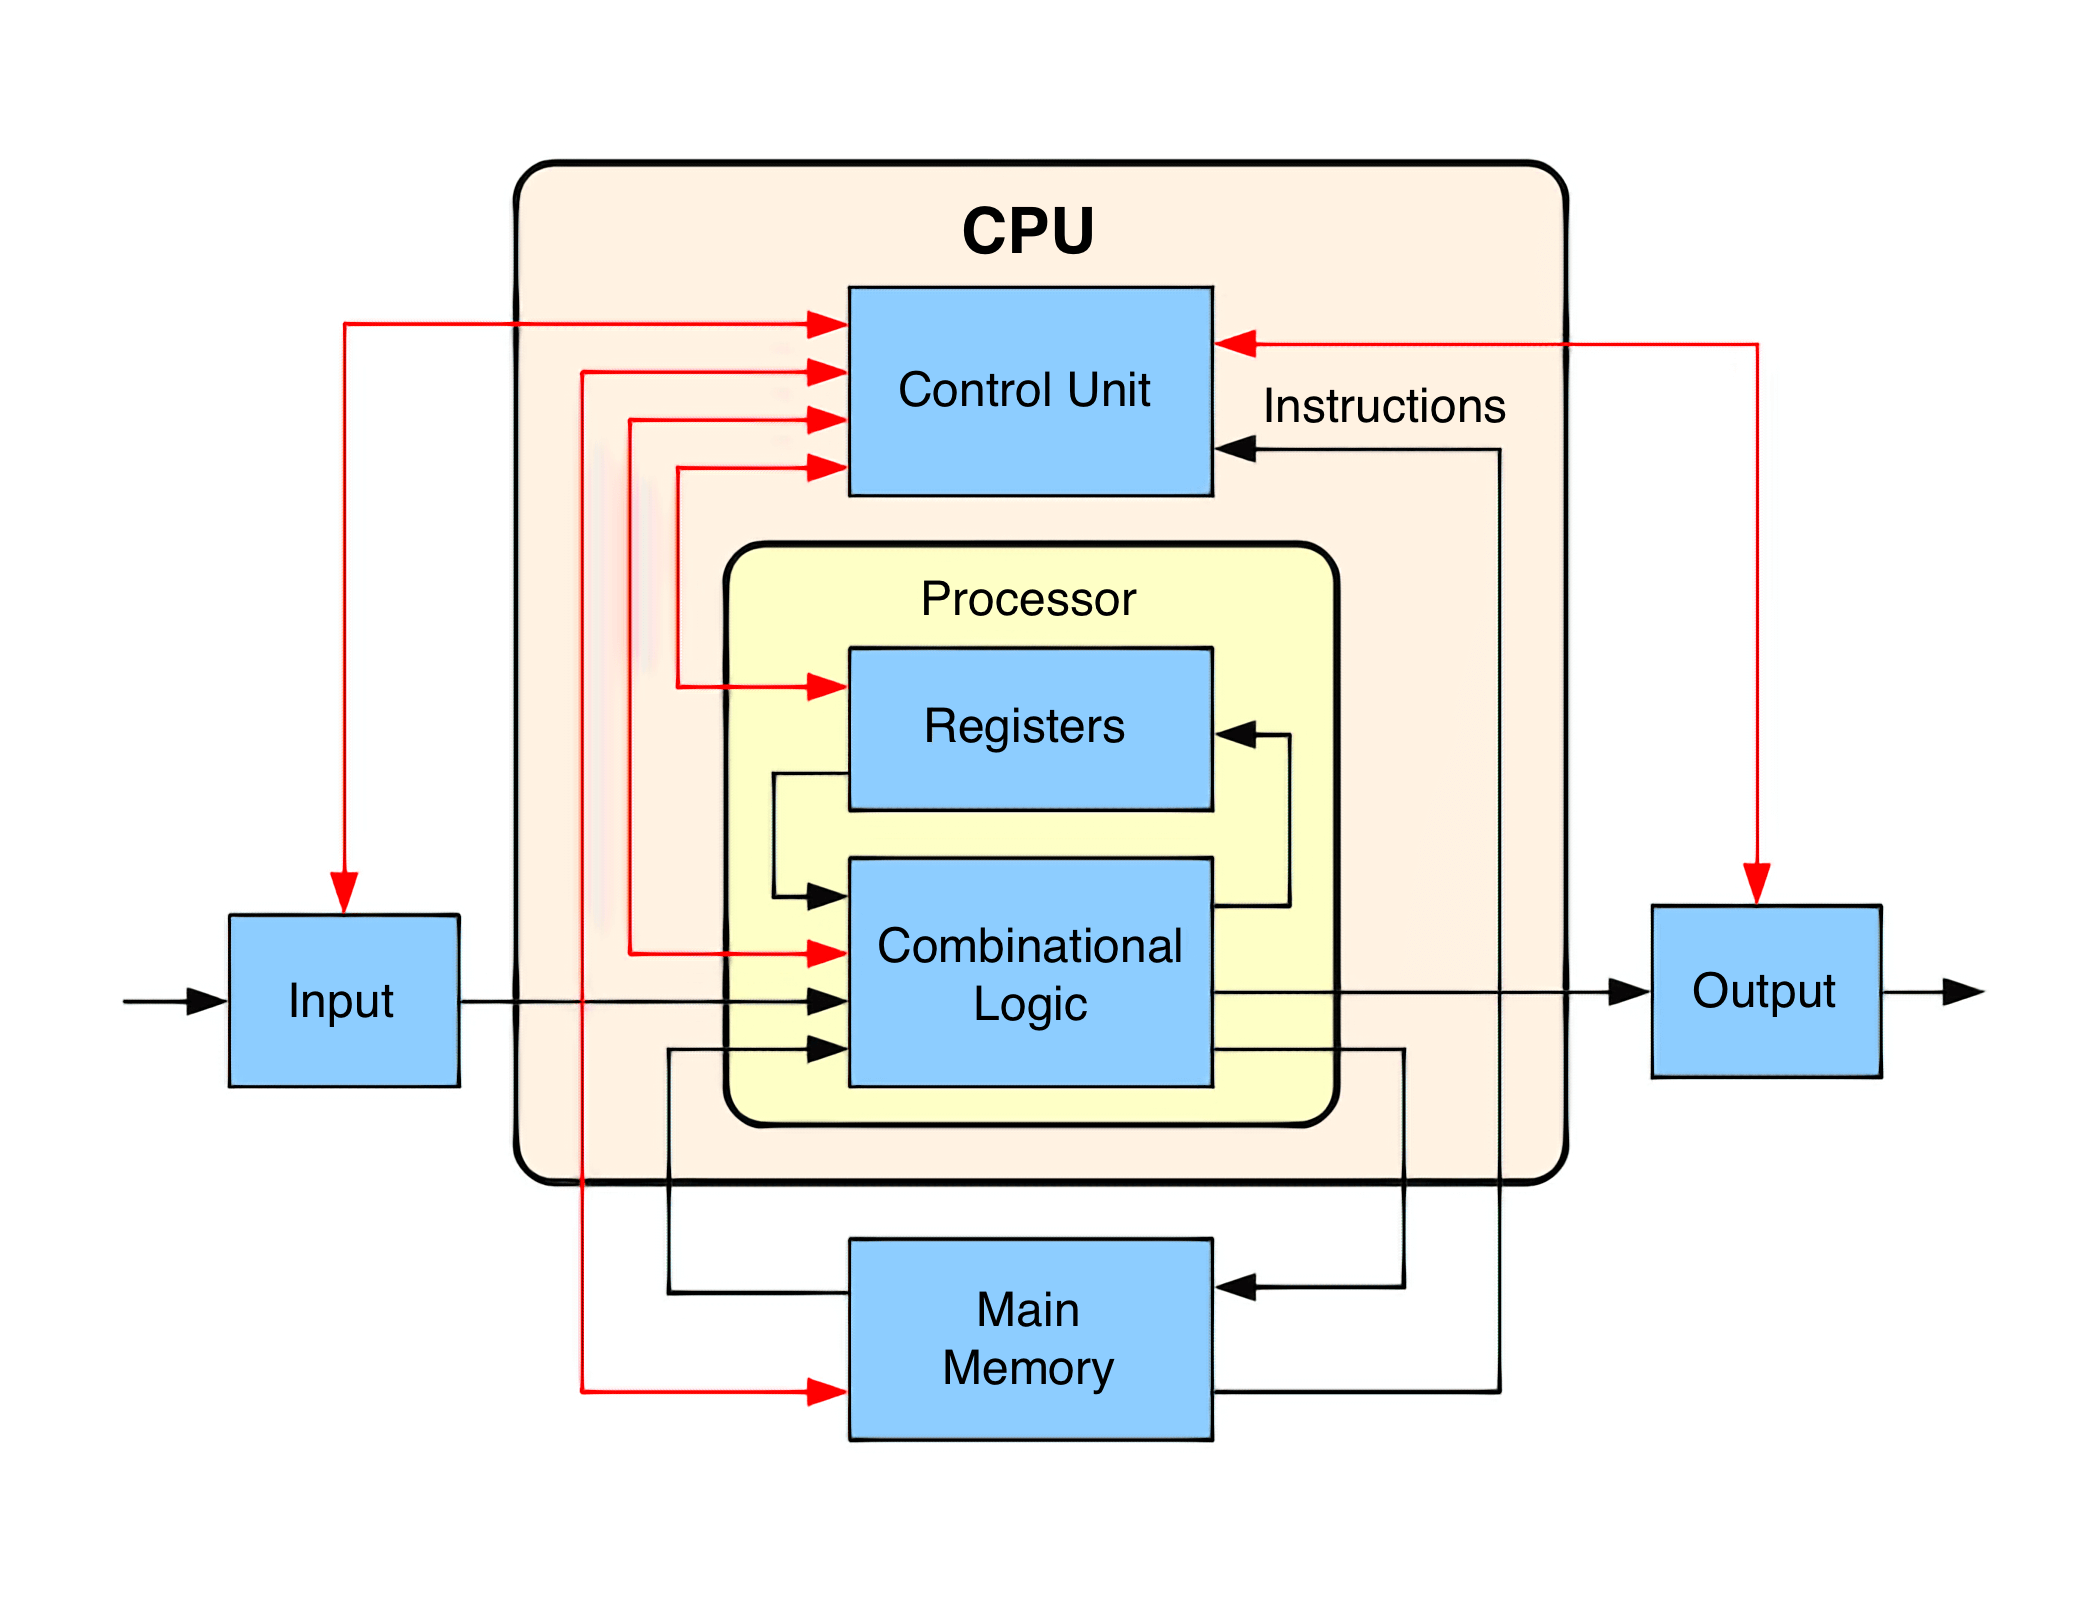
\includegraphics[scale=0.15]{cpu.png}
\end{center}

The above is an image showing the basic internals of a CPU. A CPU can be 
considered to be the primary component of a computer. It is often 
referred to as the "brain" of the computer since it is responsible
for arithmetic, logic, control and input/output operations specified by 
instructions in the computer's program. 

The two main competitors in this space are AMD and Intel. Over the years,
both have whipped out decent budget alternatives. This section will look
at what both sides can offer with respect to the aforementioned 
requirements.

\subsection{Motherboard}
\begin{center}
  % Techspot - Motherboard
  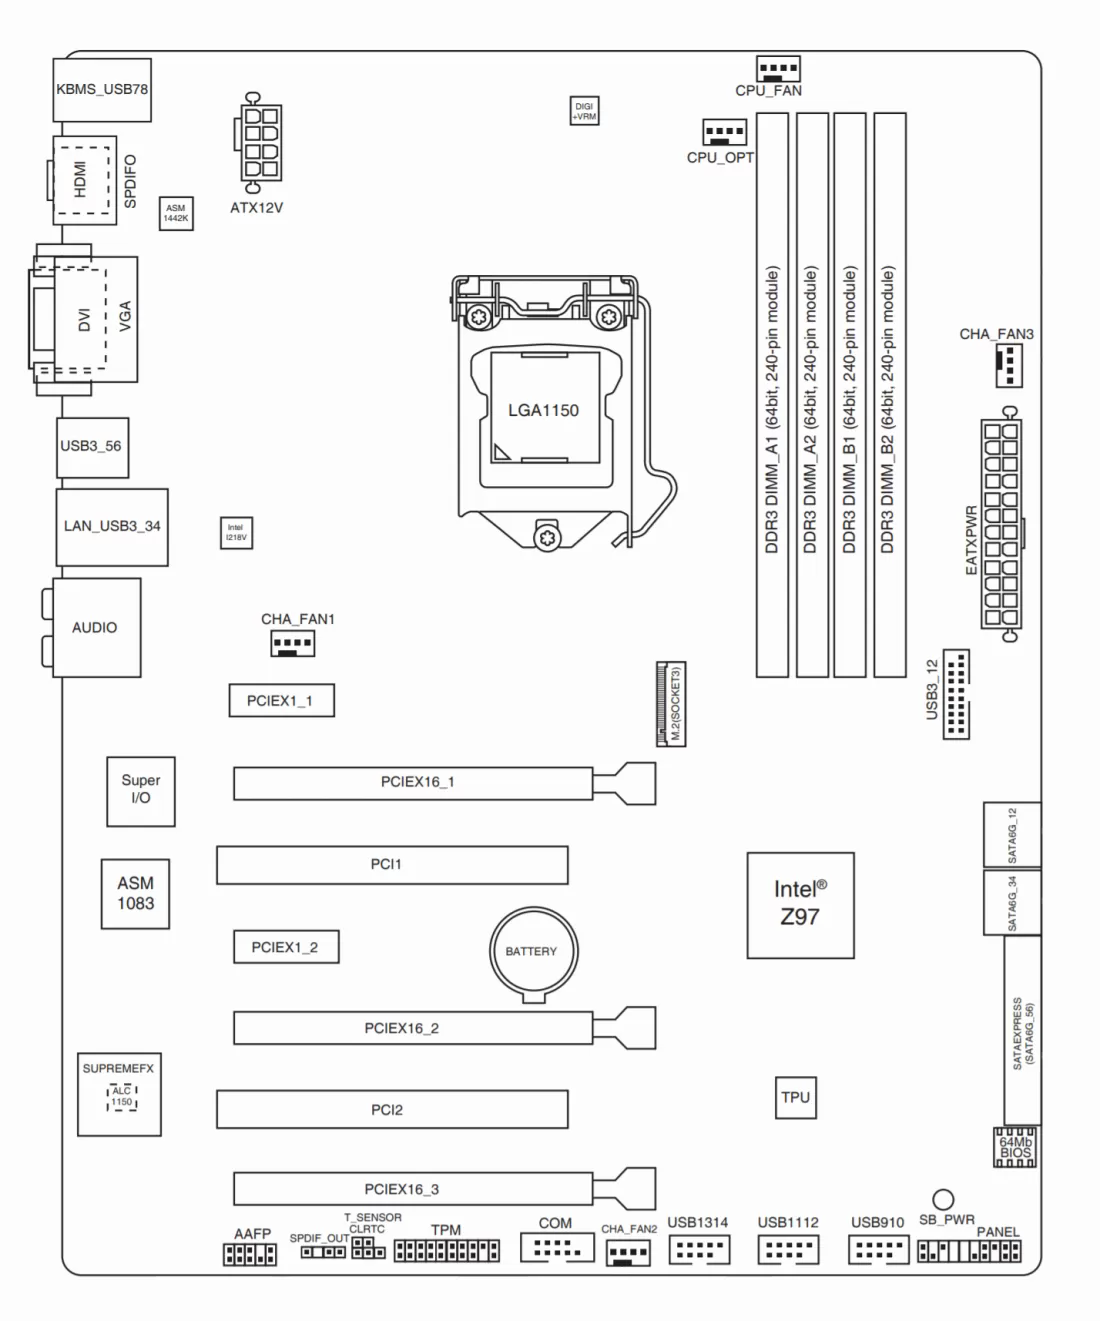
\includegraphics[scale=0.2]{motherboard.png}
\end{center}

A motherboard is the main printed circuit board (PCB) in a computer.
It serves as the foundation upon which other parts are built upon. 
It connects all the parts of the machine together. It conists of many 
parts as shown on the diagram above.

\subsection{RAM}
Random Access Memory is a form of volatile memory in a computer system
responsible for the temporary storage of data and instructions currently
being executed.

\subsection{Storage}
These include storage devices that are not directly accessible by the CPU.
They are non-volatile devices which allow data to be stored for as long
as the user needs. In terms of capacity, they are much larger than main
memory but access times are slower. Applications, the operating system,
device drivers and general files are stored in secondary storage. This
system will consider the following 2 types of secondary storage:
\begin{itemize}
  \item Hard Disk Drives: Makes use of magnetic storage technology with 
    moving parts. HDDs have slower access and data transfer speeds. They
    are also less durable and make more noise since they have 
    moving parts but are generally more affordable. 
  \item Solid State Drives: Uses flash technology and stores data in 
    non-volatile memory chips (usually NAND). They do not make use
    of moving parts and are hence quieter, smaller and more durable. 
    However they tend to be more expensive.
\end{itemize}

\subsection{Power Supply Unit}
As its name suggests, a Power Supply Unit (PSU) provides power to the 
system. In more precise terms, it converts electrical power from an outlet
to the appropriate direct current voltages required by the computer parts.
Some of its key responsibilities are: voltage regulations, provision
of connectors, modularity and safety features.

\subsection{Case}
A case provides an enclosure where other parts of the computer live in.
They come in different shapes and sizes to accommodate for different
configurations a user a opt for when building a PC. Cases serve the 
following purposes:
\begin{itemize}
  \item Protection: it protects the internal components from dust
  
\end{itemize}

\subsection{Fans}

% End Parts Investigation %

% Parts Selection %

\section{Parts Selection}

% End Parts Selection %

% Operating System %

\section{Operating System}

% End Operating System %

\end{document}

